% -*- mode: fundamental -*-

% Slides accompanying "Learn RISC-V CPU Implementation and BSV" book
% Copyright (c) 2024 Rishiyur S. Nikhil, All Rights Reserved

% -*- mode: fundamental -*-

% Slides accompanying "Learn RISC-V CPU Implementation and BSV" book
% Copyright (c) 2024 Rishiyur S. Nikhil, All Rights Reserved

% This is a preamble shared by all the slide decks

\documentclass[10pt, aspectratio=169]{beamer}

% \documentclass[17pt]{beamer}

% Avail. font sizes: 8pt, 9pt, 10pt, 11pt, 12pt, 14pt, 17pt, 20pt.
% Default font size is 11pt (= 22pt in full screen mode).

\usepackage{verbatim}
\usepackage{fancyvrb}
\usepackage{listings}

% ================================================================
% Themes

\usetheme{Madrid}          % Line at bottom: Author (affiliation), OptTitle, Conf, page 

% \usetheme{Copenhagen}    % Same as Madrid except bottom line: Author, OptTitle

% \usetheme{Berkeley}    % Takes up 1-inch border on left and top

% ----------------
% colorthemes
% (default), beaver, beetle, seahorse, wolverine

\usecolortheme{seahorse}

% ================================================================
% Customization: show table of contents before each section
% Use \AtBeginSubsection    to show before each subsection

% \AtBeginSection[]
% {
%   \begin{frame}
%     \frametitle{Table of Contents}
%     \tableofcontents[currentsection]
%   \end{frame}
% }

% ================================================================

% ----------------
% The bsc compiler and BSV language
\newcommand{\bsc}{\emph{bsc}}
\newcommand{\BSV}{\bf{BSV}}
% ----------------
% ITALICISE WORDS
\newcommand{\ie}{\emph{i.e.,}}
\newcommand{\eg}{\emph{e.g.,}}
\newcommand{\Eg}{\emph{E.g.,}}
\newcommand{\etc}{\emph{etc.}}
\newcommand{\via}{\emph{via}}
\newcommand{\vs}{\emph{vs.}}

% ----------------
% EMPTY BOXES OF VARIOUS WIDTHS, FOR INDENTATION

\newcommand{\hm}{\hspace*{1em}}
\newcommand{\hmm}{\hspace*{2em}}
\newcommand{\hmmm}{\hspace*{3em}}
\newcommand{\hmmmm}{\hspace*{4em}}

% ----------------
% Convenient widths

\newlength{\hlessmm}
\setlength{\hlessmm}{\textwidth}
\addtolength{\hlessmm}{-2em}

\newlength{\hlessmmm}
\setlength{\hlessmmm}{\textwidth}
\addtolength{\hlessmmm}{-3em}

\newlength{\hlessmmmm}
\setlength{\hlessmmmm}{\textwidth}
\addtolength{\hlessmmmm}{-4em}

% ================================================================
% Title page

\title[Learn CPU design \& BSV]{Learn RISC-V CPU Implementation and BSV}

\subtitle{(BSV: a High-Level Hardware Design Language)}

\author[{\copyright} R.S.Nikhil]{Rishiyur S.~Nikhil}
% \institute{Bluespec, Inc.}

% Date is set differently in each slide deck

% \logo{
\includegraphics[height=0.6cm]{../Figures/Bluespec_Logo_2022-10}}

% End of preamble
% ****************************************************************


\date{L5: {\BSV} Structs; Memory requests and responses}

% ****************************************************************

\begin{document}

% ================================================================

\begin{frame}
 \titlepage

 \begin{center}
  
\includegraphics[height=1cm]{Bluespec_Logo_2022-10}
 \end{center}

\end{frame}

% ================================================================

% -*- mode: fundamental -*-

% ================================================================

\begin{frame}[fragile]
\frametitle{Reminders}

\footnotesize

Please git clone: \url{https://github.com/rsnikhil/Learn_Bluespec_and_RISCV_Design} \\
(git pull for latest version).  Repsitory structure:

\vspace{1ex}

\begin{minipage}{0.5\textwidth}\scriptsize
\begin{Verbatim}[frame=single, numbers=left]
    ./Book_BLang_RISCV.pdf
      Slides/
          Slides_01_Intro.pdf
          Slides_02_ISA.pdf
          ...
      Exercises/
          Ex-03-A-Hello-World/
          Ex-03-B-Top-and-DUT/
          ...
      Code/
          src_Top/
          src_Drum/
          src_Fife/
          src_Common/
          ...
      Doc/Installing_bsc_Verilator_etc.{adoc,html}
\end{Verbatim}
\end{minipage}
\hm
\begin{minipage}{0.45\textwidth}
\begin{itemize}

 \item Slides and Exercise are numbered in sync with book Chapter numbers.

 \item For Exercises, please see Appendix E of the book.  Some (not
       all) exercises have associated code in the {\tt Exercises/}
       directory.

\end{itemize}
\end{minipage}

\vspace{2ex}

To compile and run the code for exercises, Drum and Fife, please make sure you have installed:

\begin{itemize}

 \item \emph{bsc} compiler (see \url{https://github.com/B-Lang-org/bsc})

 \item Verilator compiler (see \url{https://www.verilator.org/})
\end{itemize}

\footnotesize

\end{frame}

% ================================================================

\begin{frame}
\frametitle{Chapter Roadmap}

\footnotesize

\begin{center}
\frame{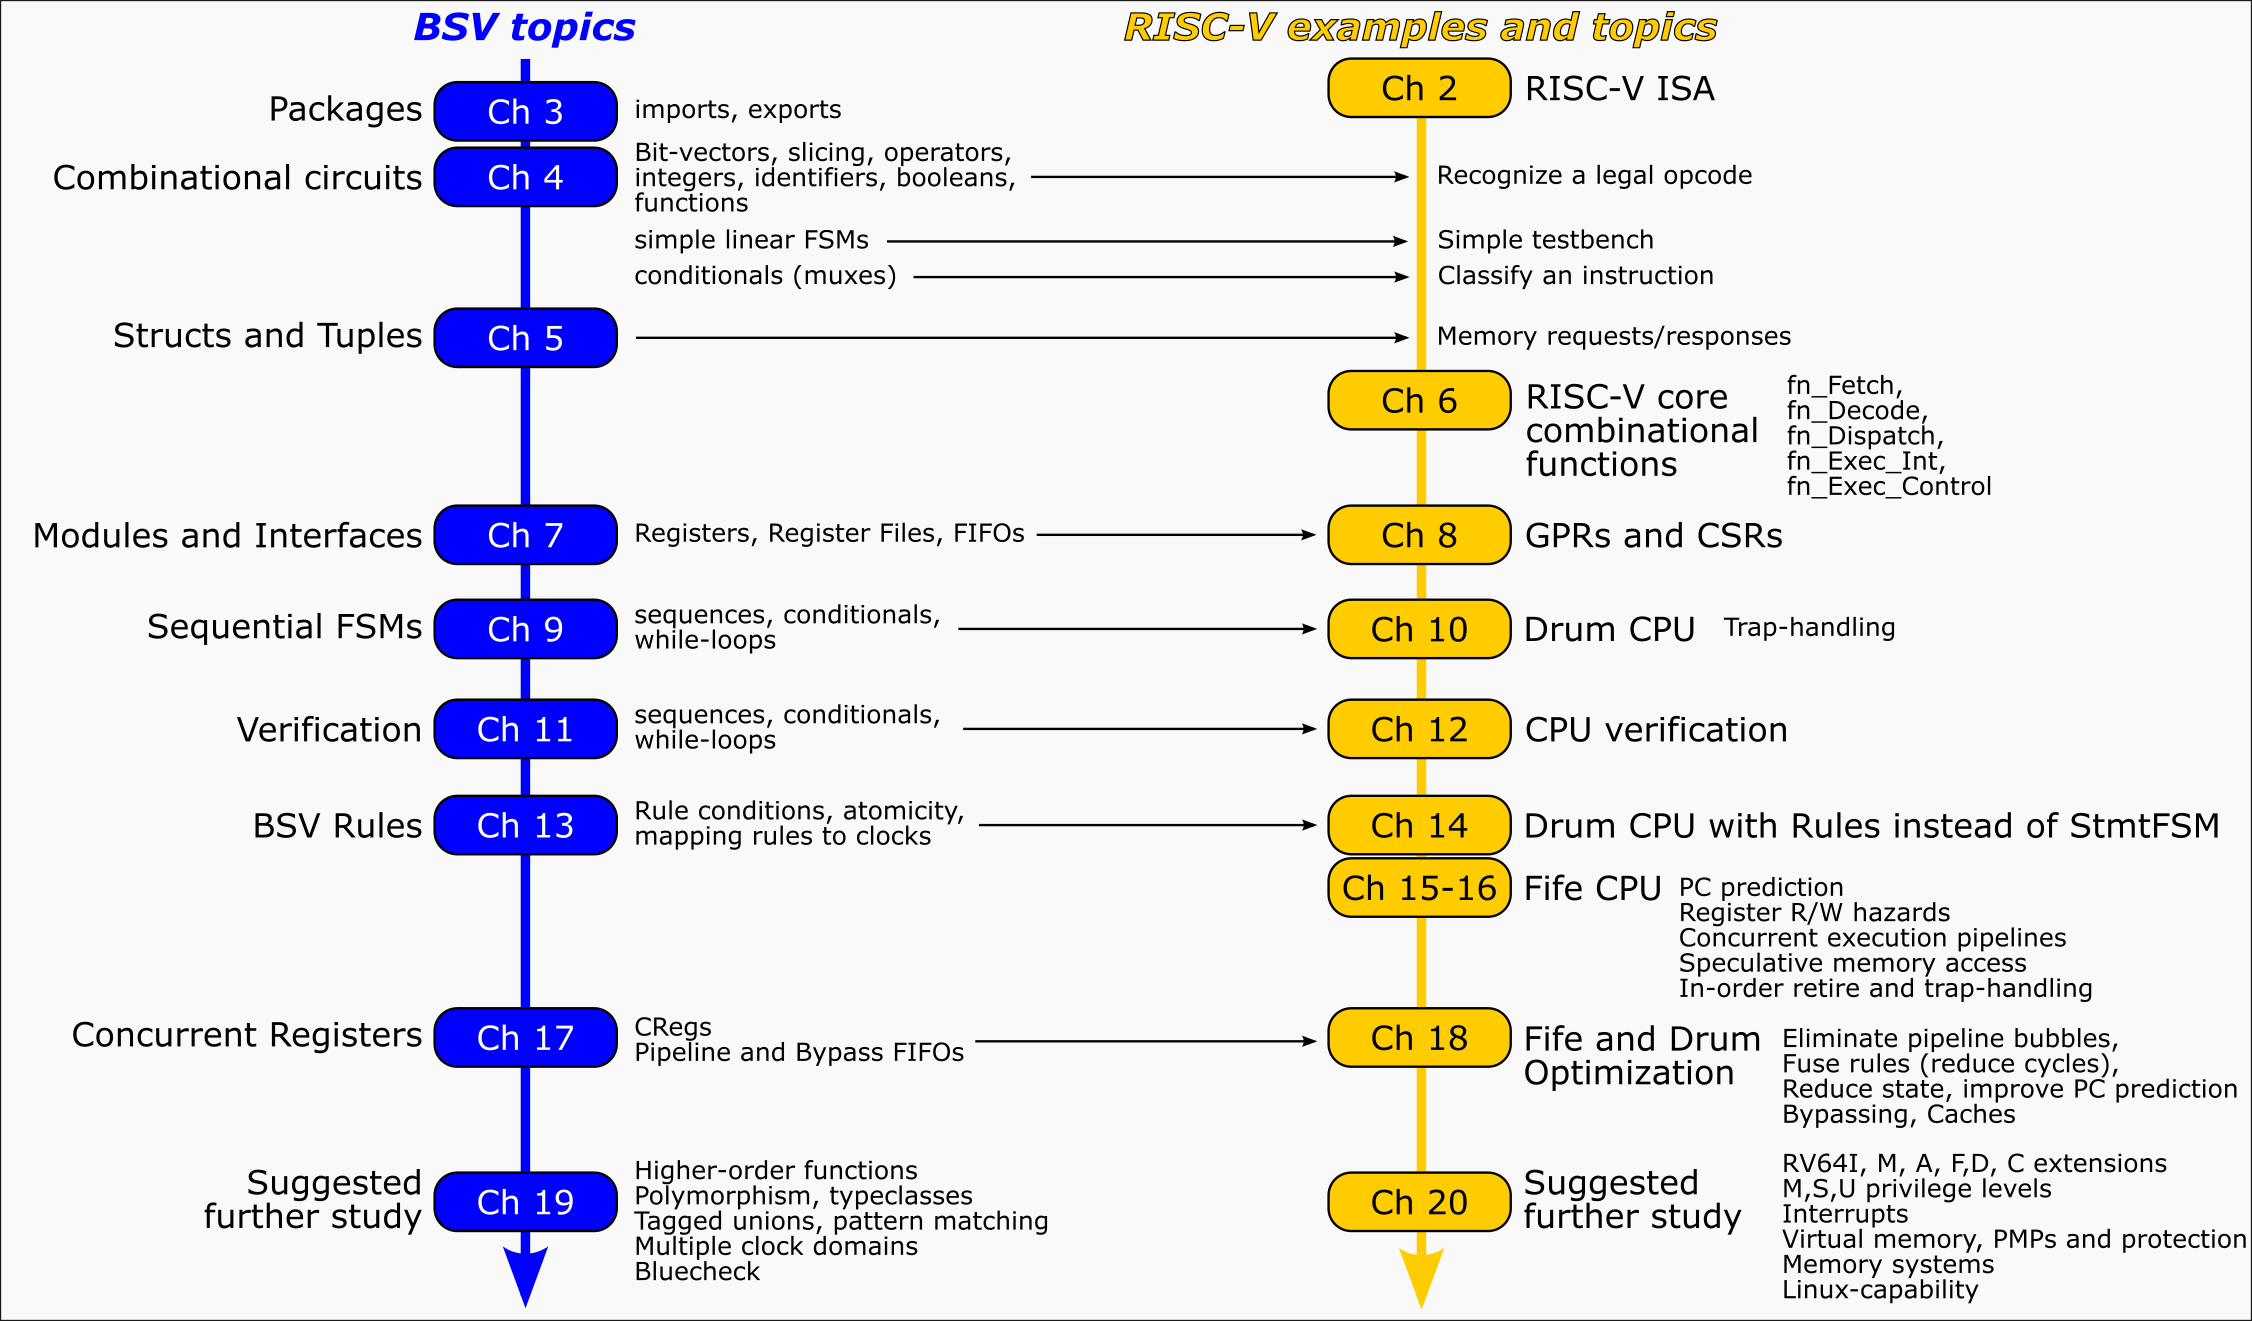
\includegraphics[height=0.825\textheight]{Fig_Chapter_Roadmap}}
\end{center}

\end{frame}

% ================================================================


% ================================================================

\begin{frame}
\frametitle{Flow of information between stages in Drum and Fife}

\footnotesize

\begin{center}
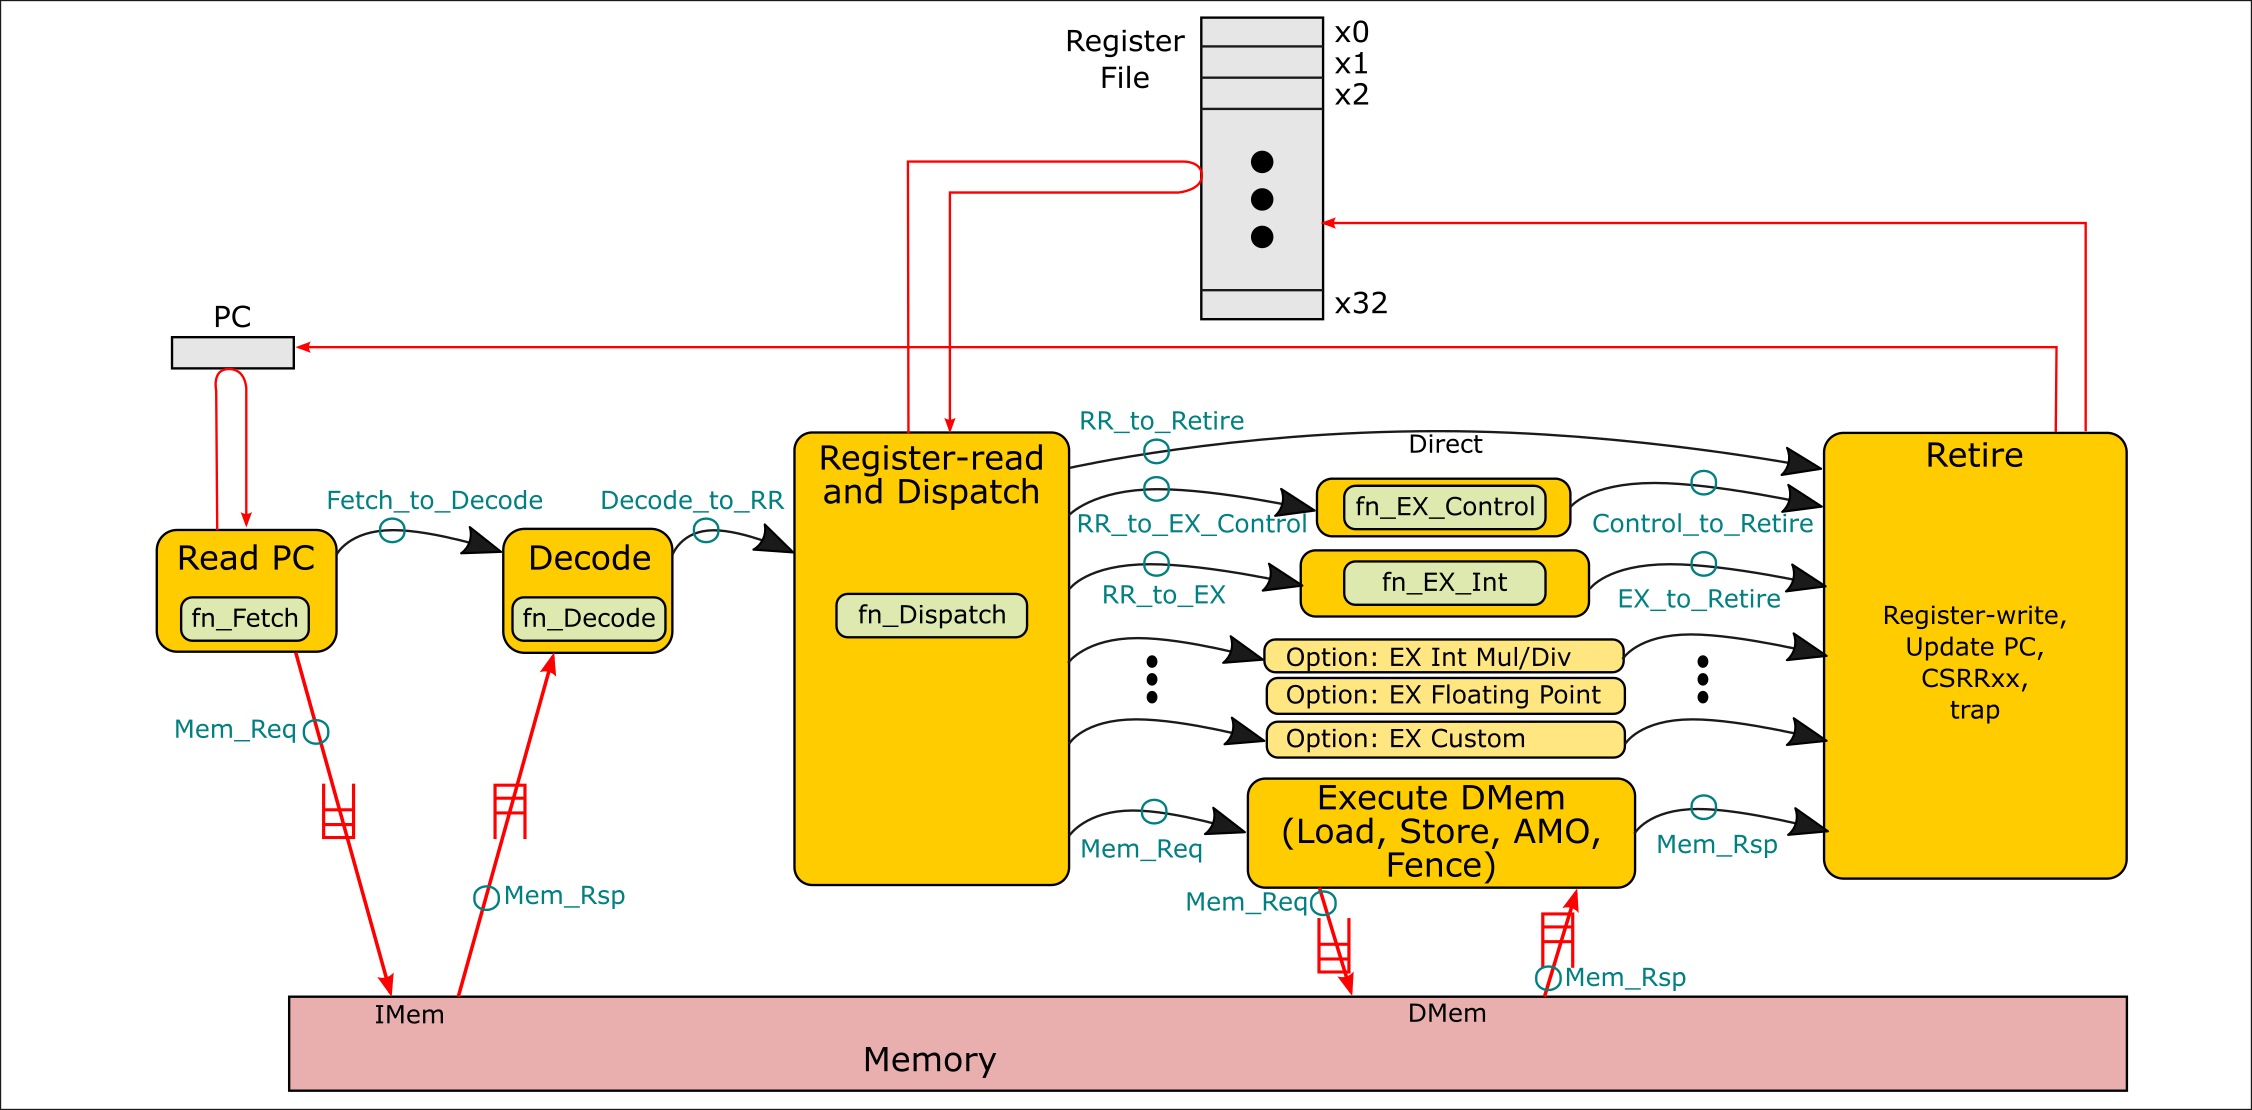
\includegraphics[height=0.6\textheight]{Fig_Instr_Exec_w_structs}
\end{center}

\vspace*{2ex}

The green annotations indicate the type of information flowing on each arrow.

Each of these is a ``{\tt struct}'' type (also known as a ``record''):
a heterogeneous grouping of \emph{fields} of various types.

\end{frame}

% ================================================================

\begin{frame}
\frametitle{Output from {\tt fn\_Decode} to the next stage}

\footnotesize

\SHOWCODE{../Code_Extracts/Decode_to_RR.tex}

\end{frame}

% ================================================================

\begin{frame}
\frametitle{Fields of struct {\tt Decode\_to\_RR}}

\footnotesize

\begin{itemize}

 \item The current PC: will be needed by BRANCH, JAL, AUIPC to compute
       a target address relative to the current PC.

 \PAUSE{\vspace{1ex}}

 \item Was there an exception (Fetch memory error, or instruction is not legal)?
       If so, what was the cause?

 \PAUSE{\vspace{1ex}}

 \item If no exception, what is the fall-through PC (needed for
       next-PC update for most instructions, and for saved-PC
       (``return address'') for JAL/JALR).

 \PAUSE{\vspace{1ex}}

 \item What is the instruction?  What is its broad classification:
       Control (Branch or Jump)? Integer Arithmetic or Logic? Memory
       Access?  This will help in choosing the execute stage pipeline.

 \PAUSE{\vspace{1ex}}

 \item Does it have zero, one or two input registers (``rs1'' and
       ``rs2'')?  If so, which ones?  This will help the Register-Read
       stage in reading registers and, for Fife, for managing ``hazards''.

 \PAUSE{\vspace{1ex}}

 \item Does it have zero or one output registers (``rd'')?  If so,
       which one?  This will help the final Register Write stage in
       writing back a value to a register.

 \PAUSE{\vspace{1ex}}

 \item Does it write memory?  In Fife, where we do speculative writes
       to memory, this will help the Retire stage commit (finalize)
       those writes.

 \PAUSE{\vspace{1ex}}

 \item What is the ``immediate'' value, if any (after untangling all
       different ways in which bits are permuted in different formats of
       instructions.

\end{itemize}

\end{frame}

% ================================================================

\begin{frame}[fragile]
\frametitle{Fields of struct {\tt Decode\_to\_RR}}

\footnotesize

Some {\tt Decode\_to\_RR} fields, such as \verb|has_rs1|, are used in
later stages, and could be computed there from \verb|instr|; so why
compute them here in Decode?

\vspace{4ex}

\begin{itemize}

 \item If something is needed in more than one stage, computing it
       once and carrying the value forward can save some hardware cost
       (gates).  It also incurs a hardware cost: we have to allocate
       state elements for the carried value in each inter-stage
       buffer/FIFO.

 \item Wherever something is computed, it adds to combinational delay
       for that stage (lowering achievable clock speed).

\end{itemize}

\vspace{4ex}

The decision between compute-and-carry {\vs} compute later is a
balancing act between these kinds of considerations.

\end{frame}

% ================================================================

\begin{frame}[fragile]
\frametitle{{\BSV}: about ``{\tt deriving (Bits, FShow)}''}

\footnotesize

\begin{itemize}

 \item Because we said ``{\tt deriving (Bits)}'', {\bsc} will
       automatically pick a hardware representation of this struct as
       a bit-vector, by simply concatenating the bit-representations
       of the fields.

 \item If we wanted a different representation, we omit ``{\tt
       deriving (Bits)}'', and there is a way (``Typeclass
       Instances'') to specify exactly what we want.

\end{itemize}

\PAUSE{\vspace*{5ex}}

\begin{itemize}

 \item Because we said ``{\tt deriving (FShow)}'', {\bsc} will
       automatically define an ``{\tt fshow()} function for this
       struct, that will print each field separately.  Otherwise {\tt
       \$display()} will simply print the flat bit-vector
       representation of the struct (which will likely be hard to
       read).

 \item If we wanted way to print the structa, we omit ``{\tt deriving
       (FShow)}'', and there is a way (``Typeclass Instances'') to
       define {\tt fshow()} to print what we want.

\end{itemize}

\end{frame}

% ================================================================

\begin{frame}[fragile]
\frametitle{{\BSV}: struct expressions to construct struct values}

\footnotesize

\begin{Verbatim}[frame=single, numbers=left]
   Decode_to_RR x = Decode_to_RR {pc:           ... value of field ... ,
                                  exception:    ... value of field ... ,
                                  cause:        ... value of field ... ,
                                  fallthru_pc:  ... value of field ... ,
                                  instr:        ... value of field ... ,
                                  ...};
\end{Verbatim}
The right-hand side is a ``struct expression'' whose value is a struct value.

\vspace{1ex}

If a field is left undefined, {\bsc} will warn while compiling.

\PAUSE{\vspace*{4ex}}

Some shorthands: ``{\tt let}'' and don't-care values:

\vspace*{2ex}

\begin{Verbatim}[frame=single, numbers=left]
   let x = Decode_to_RR {pc:           ... ,
                         exception:    False,
                         cause:        ?,
                         fallthru_pc:  ... ,
                         instr:        ... ,
                         ...};
\end{Verbatim}

\end{frame}

% ================================================================

\begin{frame}[fragile]
\frametitle{{\BSV}: Accessing and updating struct fields}

\footnotesize

These notations are standard in many programming languages.

\vspace{5ex}

\begin{Verbatim}[frame=single, numbers=left]
   x.pc
   x.instr
\end{Verbatim}

\vspace{5ex}

\begin{Verbatim}[frame=single, numbers=left]
   x.pc    = ... new value ... ;
   x.instr = ... new value ... ;
\end{Verbatim}

\end{frame}

% ================================================================

\begin{frame}[fragile]
\frametitle{{\BSV}: Tuples: pre-defined structs with special notation}

\footnotesize

Example (from {\tt mkCSRs} module in file {\tt src\_Common/CSRs.bsv}).

\vspace{2ex}

Constructing a 2-tuple value:
\begin{Verbatim}[frame=single, numbers=left]
   function ActionValue #(Tuple2 #(Bool, Bit #(XLEN)))
            fav_csr_read (Bit #(12) csr_addr);
      ...
	 return tuple2 (exception, y);
   endfunction
\end{Verbatim}

\PAUSE{\vspace{2ex}}

Accessing struct components using predefined functions {\tt tpl\_$j$}:
\begin{Verbatim}[frame=single, numbers=left]
   let xy <- fav_csr_read (...);
   let exc = tpl_1 (xy);    // exc has type: Bool
   let v   = tpl_2 (xy);    // v   has type: Bit #(XLEN)
\end{Verbatim}

\PAUSE{\vspace{2ex}}

Accessing struct components using pattern-matching:
\begin{Verbatim}[frame=single, numbers=left]
   match { .exc, .v } <- fav_csr_read (csr_addr);
\end{Verbatim}

\end{frame}

% ================================================================

\begin{frame}[fragile]
\frametitle{``Harvard'' Architecture: Separating Instruction and Data Memory}

\footnotesize

\begin{minipage}{0.35\textwidth}

 Since the very days of computers, most computers have separate channels to memory:

 \begin{itemize}

  \item ``IMem'': for Fetch to read from instruction memory

  \item ``DMem'': for LOAD/STORE instructions to read/write data memory

 \end{itemize}

 Typically, IMem and DMem can be accessed concurrently.

To facilitate this concurrency, programs typically do not modify their
 own instructions with LOAD/STORE instructions.

\end{minipage}
\hm
\begin{minipage}{0.6\textwidth}

 \begin{center}
  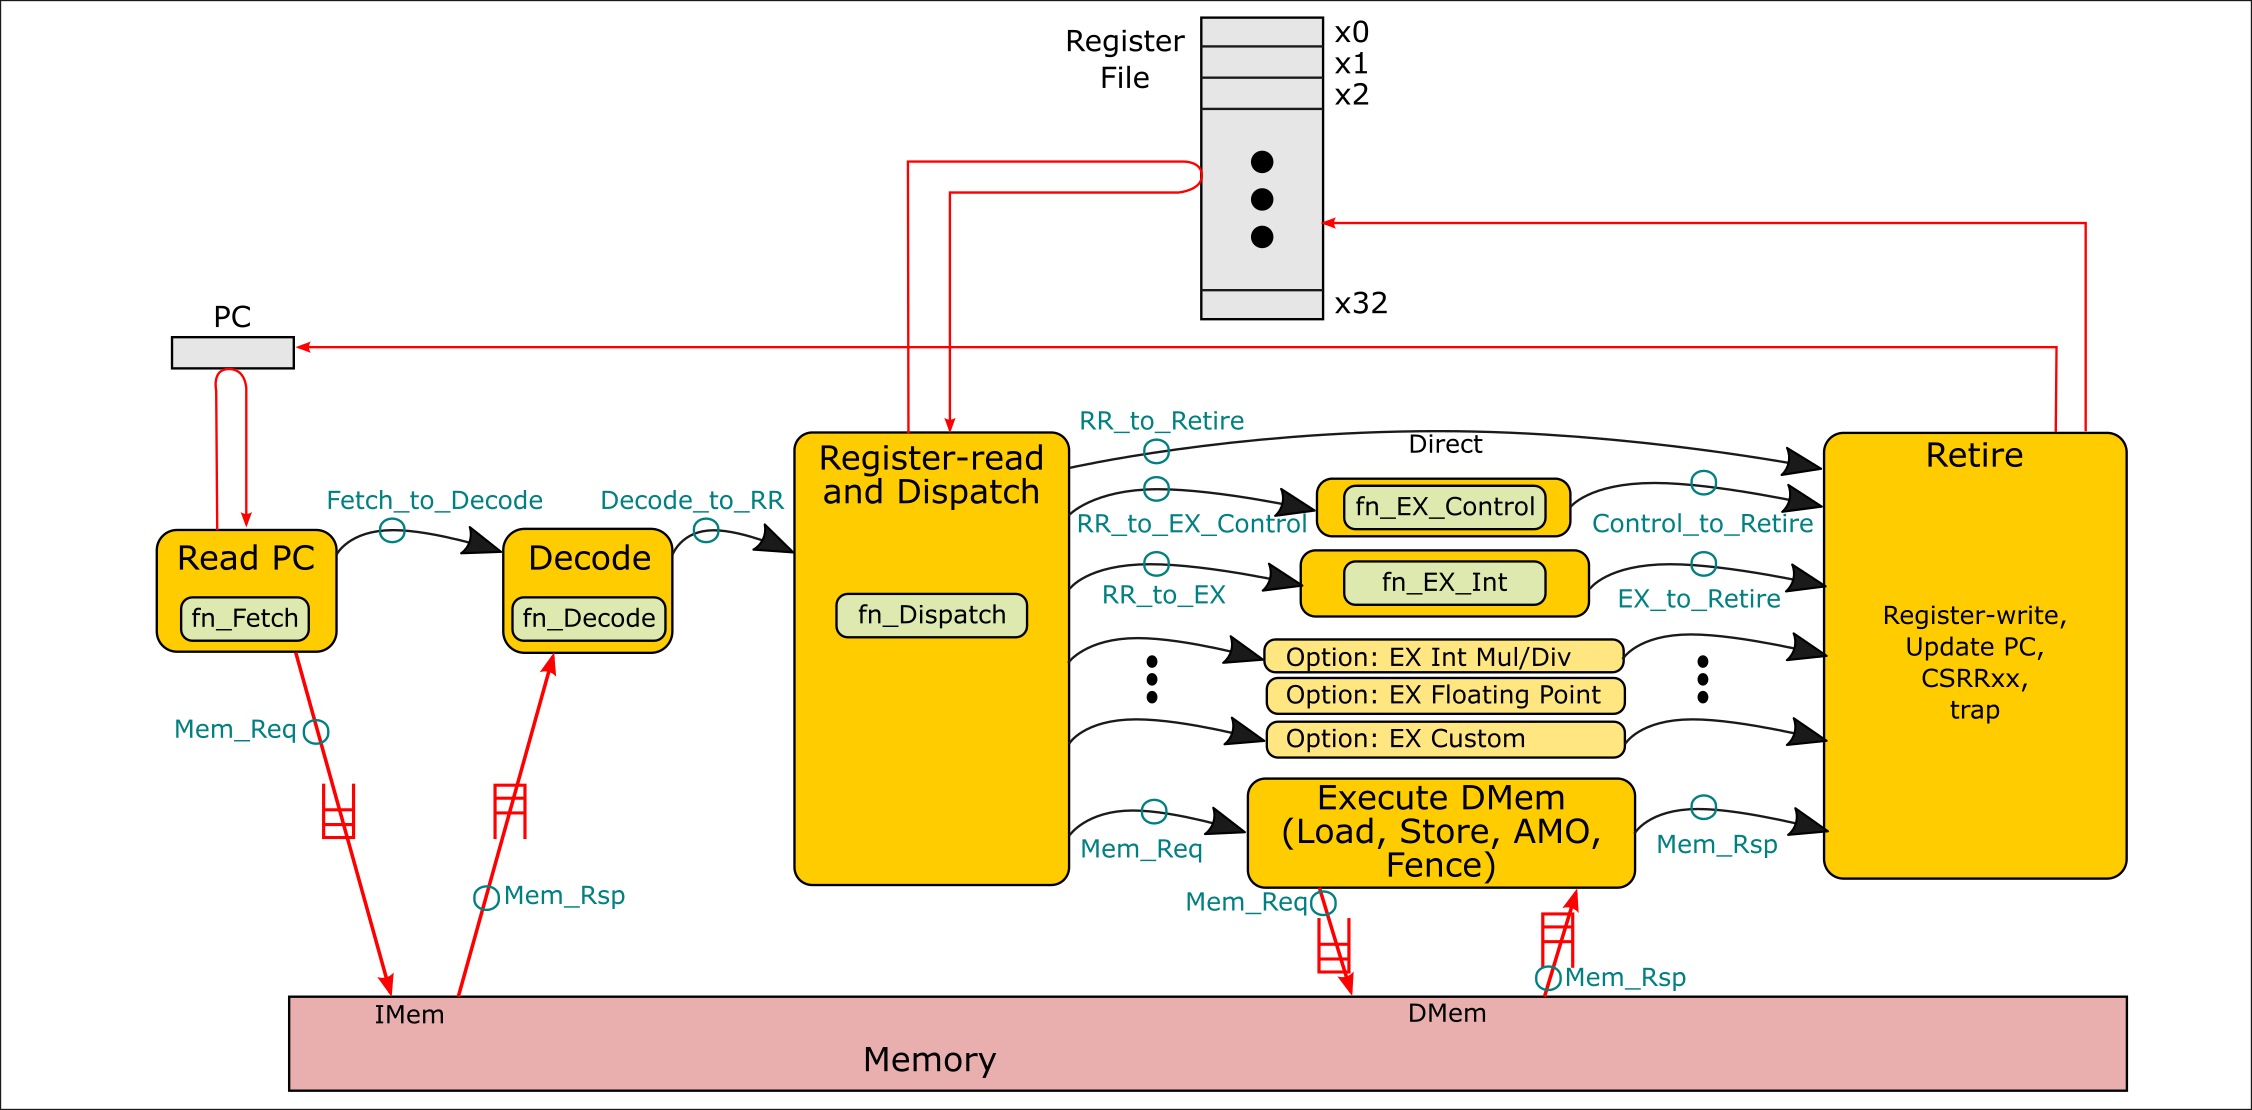
\includegraphics[width=\textwidth]{Fig_Instr_Exec_w_structs}
 \end{center}

\end{minipage}

\vfill

This organization is sometimes loosely called a ``Harvard Architecture''. \\
See: \hm \url{https://en.wikipedia.org/wiki/Harvard_architecture}.

\end{frame}

% ================================================================

\begin{frame}[fragile]
\frametitle{Memory requests}

\footnotesize

\SHOWCODE{../Code_Extracts/Mem_Req.tex}

\vspace{2ex}

We will discuss {\tt Mem\_Req\_Type} in {\tt Mem\_Req\_Size} the following slides.

\vspace{1ex}

The {\tt data} field is only relevant when communicating data from the
CPU to memory (STORE and AMO instructions).  When communicating 1, 2
and 4 bytes, these are in the least-significant bytes of the {\tt
data} field.

\PAUSE{\vspace{4ex}}

Note, we do not say ``{\tt deriving (Eq)}'' because we have no
occasion to compare two entire Memory Requests for
equality/inequality.

\end{frame}

% ================================================================

\begin{frame}[fragile]
\frametitle{Memory requests: {\tt Mem\_Req\_Type}}

\footnotesize

We could define {\tt Mem\_Req\_Type} as an {\tt enum} type ({\tt
MEM\_REQ\_LOAD}, {\tt MEM\_REQ\_STORE} ...).  However, looking ahead
to possibly supporting the ``A'' extension in the future (Atomic
Memory Ops (AMOs), see Unprivileged ISA Spec p.132), we observe that
the ISA defines a 5-bit code for each AMO op.  So, we define:

\vspace{4ex}

\SHOWCODE{../Code_Extracts/Mem_Req_Type.tex}

\vspace{4ex}

For the AMOs, we will use the 5-bit codes as defined in the ISA (simplifies Decode!). \\
For LOAD/STORE/FENCE, we use three codes that are not used by AMO ops.

\vspace{4ex}

\SHOWCODE{../Code_Extracts/funct5_MEMOPs.tex}

\end{frame}

% ================================================================

\begin{frame}[fragile]
\frametitle{Memory requests: {\tt Mem\_Req\_Size}}

\footnotesize

\SHOWCODE{../Code_Extracts/Mem_Req_Size.tex}

\PAUSE{\vspace{2ex}}

Why do we have a code for 8 bytes, since RV32I can only LOAD/STORE
bytes (1 byte), halfwords (2 bytes) and words (4 bytes)?

\PAUSE{\vspace{2ex}}

This is with an eye towards future extension of our implementation:

\begin{itemize}

 \item If we support the D ISA extension (double-precision floating
       point), we'll need to be able to load/store doublewords (8 bytes)

 \item If we support RV64I, we'll need to be able to load/store doublewords (8 bytes).

 \PAUSE{\vspace{2ex}}

 \item Even though RV32I and RV64I instructions are at most 32-bits
       wide, the Fetch stage may choose to fetch 64 bits at a time,
       effectively ``pre-fetching'' a next instruction and reducing
       the number of memory accesses.

\end{itemize}

\end{frame}

% ================================================================

\begin{frame}
\frametitle{\EmojiExercise \hmm Exercise break}

Please see directory: \hm {\tt Exercises/Ex\_05\_A\_Structs/} \\
and its README.

\end{frame}

% ================================================================

\begin{frame}[fragile]
\frametitle{Memory responses}

\footnotesize

Memory responses may report an exception (misaligned access, non-existent memory, ...).

\vspace{1ex}

\SHOWCODE{../Code_Extracts/Mem_Rsp_Type.tex}

\vspace{4ex}

\SHOWCODE{../Code_Extracts/Mem_Rsp.tex}

\vspace{1ex}

The {\tt data} field is only relevant when communicating data from
memory to the CPU (LOAD and LR instructions).  When communicating 1, 2
and 4 bytes, these are in the least-significant bytes of the {\tt
data} field.

\end{frame}

% ================================================================

\begin{frame}
\frametitle{\EmojiExercise \hmm Exercise break}

Please see directory: \hm {\tt Exercises/Ex\_05\_B\_Mem\_Req\_Rsp/} \\
and its README.

\end{frame}

% ================================================================

% -*- mode: fundamental -*-

% Slides accompanying "Learn RISC-V CPU Implementation and BSV" book
% Copyright (c) 2024 Rishiyur S. Nikhil, All Rights Reserved

% This is a postamble shared by all the slide decks

% ================================================================

\begin{frame}

\begin{center}
  {\LARGE End}
\end{center}

\end{frame}

% ================================================================


% ****************************************************************

\end{document}
